% This is the Reed College LaTeX thesis template. Most of the work 
% for the document class was done by Sam Noble (SN), as well as this
% template. Later comments etc. by Ben Salzberg (BTS). Additional
% restructuring and APA support by Jess Youngberg (JY).
% Your comments and suggestions are more than welcome; please email
% them to cus@reed.edu
%
% See http://web.reed.edu/cis/help/latex.html for help. There are a 
% great bunch of help pages there, with notes on
% getting started, bibtex, etc. Go there and read it if you're not
% already familiar with LaTeX.
%
% Any line that starts with a percent symbol is a comment. 
% They won't show up in the document, and are useful for notes 
% to yourself and explaining commands. 
% Commenting also removes a line from the document; 
% very handy for troubleshooting problems. -BTS

% As far as I know, this follows the requirements laid out in 
% the 2002-2003 Senior Handbook. Ask a librarian to check the 
% document before binding. -SN

%%
%% Preamble
%%
% \documentclass{<something>} must begin each LaTeX document
\documentclass[12pt,twoside]{reedthesis}
% Packages are extensions to the basic LaTeX functions. Whatever you
% want to typeset, there is probably a package out there for it.
% Chemistry (chemtex), screenplays, you name it.
% Check out CTAN to see: http://www.ctan.org/
%%
\usepackage{amsthm} %theorem environments etc
%\usepackage{fullpage} % reducing borders
%\usepackage{xspace}
\usepackage{amssymb} % \mathbb
\usepackage{amsmath}
\usepackage{amsfonts}
%\usepackage{hyperref}
\usepackage{graphicx}
\usepackage[vlined]{algorithm2e}
\RestyleAlgo{boxruled}

\theoremstyle{definition}
\newtheorem{dfn}{Definition}


\theoremstyle{remark}
\newtheorem*{rmk}{Remark}

\theoremstyle{plain}
\newtheorem{thm}{Theorem}
\newtheorem{lem}{Lemma}
\newtheorem{prop}{Propisition}


\newcommand{\adv}{\mathcal{A}}
\newcommand{\reals}{\mathbb{R}}
\newcommand{\gen}{\ensuremath{{\sf Gen}}\xspace}
\newcommand{\enc}{\ensuremath{{\sf Enc}}\xspace}
\newcommand{\dec}{\ensuremath{{\sf Dec}}\xspace}
\newcommand{\negl}{\ensuremath{{\sf negl}}\xspace}
\newcommand{\EXP}{\mathbb{E}}
\newcommand{\bidders}{\textbf{b}}
\newcommand{\valuations}{\textbf{v}}
\newcommand{\strategies}{\textbf{s}}
\newcommand{\OPT}{\text{OPT}}
	
	



\usepackage{graphicx,latexsym} 
\usepackage{amssymb,amsthm,amsmath}
\usepackage{longtable,booktabs,setspace} 
\usepackage{chemarr} %% Useful for one reaction arrow, useless if you're not a chem major
\usepackage[hyphens]{url}
\usepackage{rotating}
\usepackage{natbib}
\usepackage{changepage}
\usepackage{algorithmic}
\usepackage{amsthm}
\usepackage{tikz}
\usepackage [english]{babel}
\usepackage [autostyle, english = american]{csquotes}
\MakeOuterQuote{"}

\graphicspath{./diagrams/}
% Comment out the natbib line above and uncomment the following two lines to use the new 
% biblatex-chicago style, for Chicago A. Also make some changes at the end where the 
% bibliography is included. 
%\usepackage{biblatex-chicago}
%\bibliography{thesis}

% \usepackage{times} % other fonts are available like times, bookman, charter, palatino

\title{Simulating Auctions}
\author{Robert S. Irvin}
% The month and year that you submit your FINAL draft TO THE LIBRARY (May or December)
\date{May 2020}
\division{History and Social Sciences}
\advisor{Jeffery Parker}
%If you have two advisors for some reason, you can use the following
\altadvisor{David Perkinson}
%%% Remember to use the correct department!
\department{Economics and Mathematics FIXME}
% if you're writing a thesis in an interdisciplinary major,
% uncomment the line below and change the text as appropriate.
% check the Senior Handbook if unsure.
%\thedivisionof{The Established Interdisciplinary Committee for}
% if you want the approval page to say "Approved for the Committee",
% uncomment the next line
%\approvedforthe{Committee}

\setlength{\parskip}{0pt}
%%
%% End Preamble
%%
%% The fun begins:
\begin{document}

  \maketitle
  \frontmatter % this stuff will be roman-numbered
  \pagestyle{empty} % this removes page numbers from the frontmatter

% Acknowledgements (Acceptable American spelling) are optional
% So are Acknowledgments (proper English spelling)
    \chapter*{Acknowledgements}
	The cat, Pinoe.

% The preface is optional
% To remove it, comment it out or delete it.
    \chapter*{Preface}
	This is an example of a thesis setup to use the reed thesis document class.
	
	

    \chapter*{List of Abbreviations}
		You can always change the way your abbreviations are formatted. Play around with it yourself, use tables, or come to CUS if you'd like to change the way it looks. You can also completely remove this chapter if you have no need for a list of abbreviations. Here is an example of what this could look like:

	\begin{table}[h]
	\centering % You could remove this to move table to the left
	\begin{tabular}{ll}
		\textbf{AI}  	&  Artificial Intelligence\\
		\textbf{MAS}  	&  Multi-Agent System\\
		\textbf{MDP}    &  Markov Decision Processes\\
		\textbf{ML}     &  Machine Learning\\
	\end{tabular}
	\end{table}
	

    \tableofcontents
% if you want a list of tables, optional
    \listoftables
% if you want a list of figures, also optional
    \listoffigures

% The abstract is not required if you're writing a creative thesis (but aren't they all?)
% If your abstract is longer than a page, there may be a formatting issue.
    \chapter*{Abstract}
	The preface pretty much says it all.
	
	\chapter*{Dedication}
	You can have a dedication here if you wish.

  \mainmatter % here the regular arabic numbering starts
  \pagestyle{fancyplain} % turns page numbering back on

%The \introduction command is provided as a convenience.
%if you want special chapter formatting, you'll probably want to avoid using it altogether

    \chapter*{Introduction}
         \addcontentsline{toc}{chapter}{Introduction}
	\chaptermark{Introduction}
	\markboth{Introduction}{Introduction}
	% The three lines above are to make sure that the headers are right, that the intro gets included in the table of contents, and that it doesn't get numbered 1 so that chapter one is 1.

% Double spacing: if you want to double space, or one and a half 
% space, uncomment one of the following lines. You can go back to 
% single spacing with the \singlespacing command.
% \onehalfspacing
\doublespacing
	
	This thesis will lay out the literature on the price of anarchy bounds for single item, first price auctions and then will construct a simulation to demonstrate these bounds for no-regret agents. Chapter one hopes to be a broad overview of the field to give context for this discussion covering price of anarchy, auctions, and simulation. Chapter two will go through the mathematical theory in a more rigorous way laying out what sort of behavior we expect and why for no-regret agents in these auctions as well as how the price of anarchy for first price, single payer auctions were derived. Chapter three will be the empirical results of a simulation which hopefully accord with what the theory says. 
	
	\textbf{Note to the readers of this draft of chapter 1}: the in-text citations generated by Latex are formatted incorrectly/in the wrong style for this draft and I will talk to CUS to try and get this fixed. These will look like (Author1 \& Author2 (year)) which is incorrect.

\chapter{Computational Economics and Auctions}
	Within the last three decades, computational economics has been on the rise. This branch of economic research encompasses two major ideas. One is that the increasing power of computers can help solve and understand classical economic problems through increasingly more complex simulations and numerical analysis. Two, that the mathematical methods developed in the field of theoretical computer science can be used to gain better understanding of existing models in terms of their algorithmic and computational complexity properties. We aim to take elements from both of these frameworks to better understand the social welfare of auctions at equilibrium. 

\section{Auctions, Equilibria, and Anarchy}
It is perhaps obvious why economists would be inserted in studying auctions. Auctions are one of the most basic market structures that have roots going back to at least the ancient Greeks and still exist today in places such as art auctions and Ebay (\cite{Mochon2015}). But in the past 15 years, economists have been joined by computer scientists who are increasingly interested in the strategic interactions of agents within this setting. Christos Papadimitriou said in a 2015 lecture at the Simons Institute that it was the advent of the internet, an artifact out of their control, that turned theoretical computer science into a "physical science." Now computer scientists had to "approach the internet with the same humility that economists approach the market..." He went on to say that "it also turned us [computer science] into a social science. It was obviously about people and incentives. Without understanding this, you cannot understand the internet" (\cite{Papadimitriou2015}). It is within this framework that computer scientists first began to study auctions as they existed on the internet. At first, this meant trying to understand the auctions present there such as Ebay and Googles sponsored search auctions. But now, they are moving beyond that and taking the mathematical tools of theoretical computer science and applying them as a lens to understand and explain the world beyond the scope of the internet. Here specifically we are looking at the field algorithmic game theory, the study of the algorithms and complexity of strategic interactions. For economists, this can be thought of as a new toolbox for unpacking and understanding the models and structures that already dominate the field. For example, in the case of a Walrasian auctioneer who calculates the clearing prices of a combinatorial auction, their problem was shown to be NP-complete, a complexity class usually called "intractable" due to the time it takes to solve these problems (the best algorithms here are generally guess and check, which gets out of hand for large inputs i.e. possible combinations) (\cite{Papadimitriou2015})\footnote{NP is the class of problems that a given solution can be checked in polynomial time, i.e. $O(n^k)$ operations where $n$ is the size of the input and $k$ is any positive integer. NP-complete means that all problems in NP reduce to solving this problem. This is when you will usually hear "taking more time to compute then the age of the universe" etc...}. Using the lens of computational complexity is one way of assessing what assumptions we are making about the computational power of our rational agents.

\subsection{The Price of Anarchy}
Another idea that has come out of algorithmic game theory is the price of anarchy (POA), a mathematical way of showing the difference between the social welfare in the optimal case and in the worst case equilibrium for a game. More formally, the price of anarchy for a game is the ratio of the minimum equilibrium social welfare in a game over the best possible social welfare of the game. An illustrative example of the price of anarchy can be seen in selfish routing games such as the one pictured below in figure \ref{braess} that comes from Tim Roughgarden's 2016 book "20 Lectures on Algorithmic Game Theory". 
\begin{figure}[h!]
	\centering
	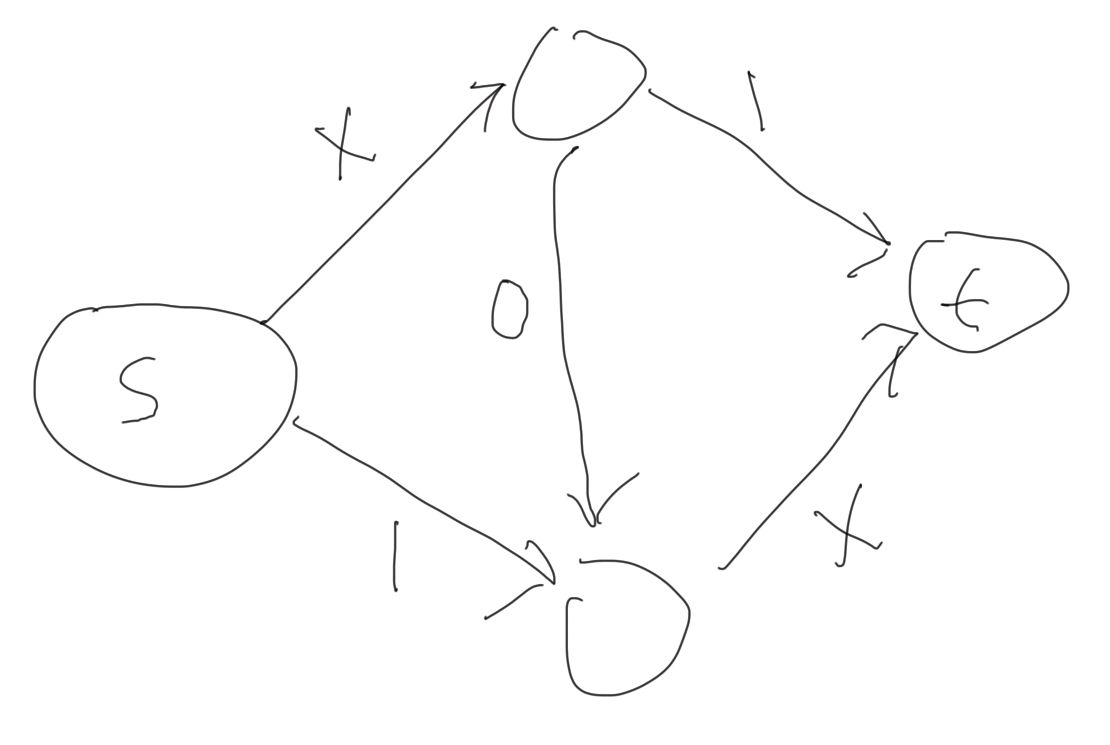
\includegraphics[scale=0.4]{braess}
	\caption{Routing game from s to t. Strategic interaction will make everyone worse off.}
	\label{braess}
\end{figure}
In this game, each player chooses which edges to take on the directed graph from the source $s$ to reach the terminal $t$ and try to do it in the least time, total weight of edges taken, as possible. For the edges labeled x, x is equal to the proportion of players who take the route.\footnote{These figures are slightly off. The edges should have weights $f(x) = x$ or $f(x) = 1$ giving us the cost of using the edge as a function of the proportion of people who are using that edge. This will be fixed when I draw these graphs properly for the final draft and not in MS paint.} For example if $50 \%$ of the players take that edge then $x=0.5$. This can be seen as analogous to traffic when driving a car, the more people take a road, the slower the traffic goes and the longer it takes to get somewhere. Knowing this, each player must choose which path to take to get to their destination as quickly as possible. As you can quickly verify, the best solution for society, minimizing the total driving time for all, is when half of the drivers take the top route, and half of the drivers take the bottom route taking in total 1.5 for each driver. 

\begin{figure}[h!]
	\centering
	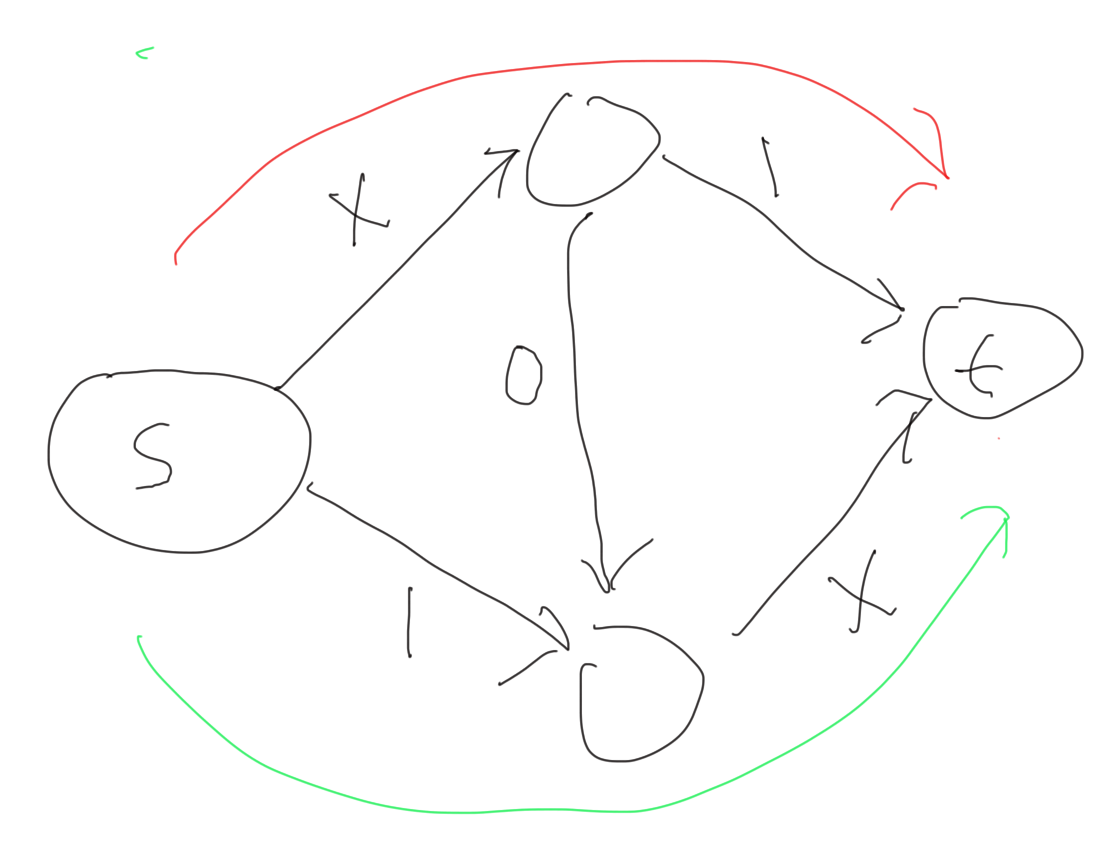
\includegraphics[scale=0.4]{braess_2}
	\caption{Socially optimal route: half taking top, half taking bottom}
	\label{braess2}
\end{figure}

However, this is not an equilibrium. The drivers taking the top route have incentive to instead take the middle edge to try and lower their total time traveled. In fact, the Nash equilibrium will end up with all of the drivers taking the top x, going through the middle, and then the bottom x. Only then will no players have reason to deviate. These actions to individually and strategically try to decrease their cost end up producing a worse outcome for all players and society as a whole (the social welfare)\footnote{A careful observer will note that if the edge with cost 0 were not there, this would not be a problem. This is called Braess's Paradox where having this extra edge counter intuitively leads to worse outcomes. (\cite{Roughgarden2016})}.  

\begin{figure}[h!]
	\centering
	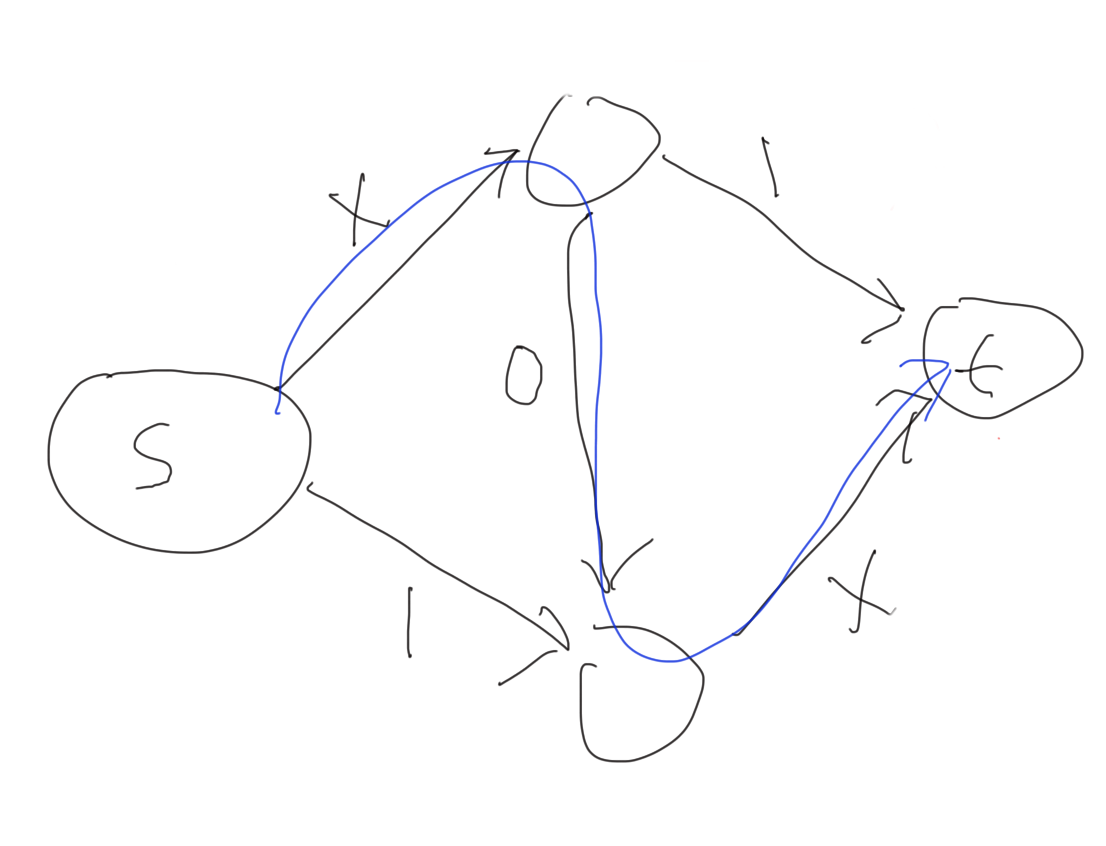
\includegraphics[scale=0.4]{braess_3}
	\caption{Route under strategic interaction}
	\label{braess3}
\end{figure}

Now, it will take time 2 for each player to reach the terminal. Thus, under strategic interaction we see that the equilibrium is sub-optimal for society, and in this case all players as well. In this case, the price of anarchy can be computed as $$POA = 3/4$$. Interestingly, bounds for the price of anarchy can be found for the class of game as a whole regardless of its individual construction. The price of anarchy bound for these selfish routing games is know to be $3/4$, meaning that our example is as bad as the price of anarchy could get for any selfish routing game.

\subsection{Auctions}
This framework of the price of anarchy is now being applied to understand auctions by researchers in the algorithmic game theory field. Where for selfish routing games, the price of anarchy has been shown to have the tight bound above, the price of anarchy for single price auctions only has approximate upper and lower bounds set on it, and is not known at all for double auctions. Before exploring this further, we should set up the mathematical framework of auctions that is necessary to compute such bounds. 

An \textbf{auction} is a market mechanism, operating under specific rules that determines to whom one or more items will be awarded and at what price. For a bidder in an auction, the \textbf{value} $v_i$ is how much the bidder values the item. This is sometimes called a private valuation as this value is generally unknown by the other participants in the auction. The \textbf{bid}, $b_i$, is the offer that bidder $i$ submits for for an item. \textbf{Sincere bidding} is when $v_i = b_i$, \textbf{underbidding} is when $v_i > b_i$, and \textbf{overbidding} is when $v_i < b_i$. The highest bid made by any bidder is denoted $b^*$, and is the winning bid (if multiple bids equal the winning bid, then some tie-breaking rule must be used). The \textbf{selling price}, $p^*$ is the final price that the bidder actually pays for the item (which depending on the auction type need not equal $b^*$). Under the \textbf{first-price} rule, the bid submitted by the winner is equal to the selling price. Before the auction begins, each bidder knows their personal or private value for the item. An auction consists of a set of bidders, $I = (1,2, ...,N)$ and a seller. After the auction, the bidder $i$ wins the item if their bid is higher than the bid placed by any other bidder $k$, $b_i > max_{k \neq b_k}$. In a single unit auction, the \textbf{income of the bidder} $i$ is equal to their value of the item: $$ \Gamma_i^* = v_i$$ and the \textbf{surplus of the bidder} $i$ is equal to the difference between income and price paid $$ \Pi_i^* = \Gamma_i^* - p^*.$$ If a bid placed by a bidder is less than the winning bid, they do not win anything and their income and surplus are both zero. The \textbf{seller's revenue} in a single unit auction is equal to the price paid by the winning bidder $$ R^* = p^*.$$ 

There are multiple different pricing rules in an auction that determine who gets allocated the item. In a \textbf{First-Price} auction the winning bidder pays the amount of their bid, which is the highest bid of the auction: $p^* = b^*$. Also called \textbf{pay-what-you-bid} (PWYB). In a \textbf{Second-price} auction, the winning bidder pays an amount that is equal to the second highest bid for the awarded item \cite{Vickrey1961} \footnote{The second price, sealed bid auction is also known as a Vickrey auction after the economist who invented it}. People tend to bid lower than their private valuation in first price auctions since if they bid that value, their profit is zero. Thus, the first price rule the item could be awarded to someone who values the item less than other bidders. Second price auctions encourages bidder to bid their true values (as they will gain positive profits if they win no matter the second highest bid). This encourages an efficient allocation of items (\cite{Mochon2015}). For the moment we will confine ourselves to first price auctions as this is where most of the strong results in POA analysis of auctions currently are.

Before discussing the known bounds on the price of anarchy for first price, single payer auctions, it is worth understanding how the bids might lead to a non-optimal outcome or what we mean by that. Due to only knowing their own valuation of the good, each bidder must act under uncertainty as to how much they should bid to beat out the unknown valuations of the other bidders. However, if they bid their exact private valuation then they will get a surplus of zero, or zero utility. In order for them to get some utility for the item they must be paying less then the exact amount they value the item. How much each bidder should bid less than their valuation, or "shade", their bid is determined by how much they think that the other party values the item. To capture this interaction auctions are represented as Bayesian games where each bidder is drawing their bids from distributions known to the other player (that need not be the same). If one player knows that the other is drawing from a distribution with a smaller mean than they are (i.e. probably doesn't value the item as much), the Bayes-Nash equilibrium will have them shade their bid less and this other person will shade their bid more. This can lead to the person who values the item less winning the auction and creating less social welfare (the summed surplus of all bidders and the seller). 

Syrgkanis and Tardos proved in 2013 that the price of anarchy in first price, single item auctions is at least $1 - \frac{1}{e} \approx 0.63$. The exact upper bound on the price of anarchy for single payer, first price auctions remains unknown in the general case. This bound is true regardless of how many bidders there are or what distributions they are drawing their bids from.

This moves closer to answering the question for what is the price of anarchy at equilibrium, but these results do not pay attention to how the players arrive at these equilibria. In real world applications, we expect that players might play repeatedly in the same auction and learn as they play rather than come in with pre-computed strategies. This is especially true for when computing the equilibrium is computationally hard and the stakes of each individual auction is small. Given these observations, it is natural to ask questions about how the efficiency results carry over to adaptive game environments. The model for learning agents that is commonly used in the field is \textbf{no-regret learning}. An algorithm for a player satisfies the no-regret condition if, in the limit as the number of times the game is played goes to infinity, the average reward of the algorithm is at least as good as the average reward for the best fixed action in hindsight (assuming the sequence of actions for the other players remains unchanged)\footnote{That is to say that the algorithm will converge to having a loss no worse than any fixed strategy we would have rather picked in hindsight as the limit goes to infinity. A more precise definition, example algorithms, and uses will be shown in chapter 2 to clarify what "regret" is and how this converges to zero}. If each player  incorporates this kind of learning algorithm, then it has been shown that these can converge to a larger class of equilibrium called correlated equilibrium where each player conditions their response on the expected action of the other player. Luckily, the previous theorem has been extended so that we know that the price of anarchy for the correlated equilibria of first price auctions are also at least 0.63 (\cite{Roughgarden2017})

With all of this set up, we now state our goal: to simulate no-regret learning algorithms for agents in a first price, single payer auction to see how well the price of anarchy holds. We also want to compare this with other learning algorithms that aren't no regret to see if this framework of using these algorithms is appropriate for making generalizations about equilibrium under learning.

	
\section{Simulated Agents and Simulated Economies}
The use of computers in economics goes back all of the way to general purpose computers being invented in the 1940's. Wassily Leontif used a computer to invert a 39 x 39 matrix to help solve his input output model. Since then, computers use in economics has exploded. With computers, economists are able to solve bigger matrices, do Monte-Carlo simulations, create multinomial probit models, and use full information maximum likelihood estimation (\cite{Backhouse2016}). While one branch of computational economics is focused on creating stronger and stronger calculators to facilitate empirical research, another branch has focused on creating simulated economies that allow economists to construct a blended version of theory and research within a computer program. Within these simulated economies, theories can be coded into the simulation which, when run, can allow the researcher to conduct experiments that might not be practical to conduct in the real world. 

One kind of a simulation that can be run is called an agent-based model (ABM), a simulated system of autonomous decision makers (agents). These models are able to generate complex behavior even if only simple assumptions are made about the behavior of the coded agents. That is, these agents interacting with each other in complex ways are able to produce emergent phenomena in the macro structure of the system.

For example, in the 1970's Thomas Schilling created a computer simulation to try and understand how and why self segregated neighborhoods formed. He coded a virtual environment where agents were given a simple preference, they are only happy if they are not the minority in their neighborhood and will keep moving otherwise. This simple model can illustrate the main tenets of agent based modeling. First, we have agents who are representative of people in the real world. Their preferences to this respect are simple and easy to understand where they are only "happy" if half of their closest neighbors are the same as them. If they are not happy they will move somewhere else arbitrarily. These preferences can be represented as the short procedure, or algorithm, shown below where $S$ is just the space they live in.

\begin{adjustwidth}{1cm}{}
	\textbf{1.} Draw a random location in $S$ \\
	\textbf{2.} If happy at new location, move there\\
	\textbf{3.} Else, go to step 1
\end{adjustwidth}

In this case, we get to choose what that environment looks like and like Shelling we can just say that it is a one by one unit square and we can say that their neighbors are the ten closest people to them (in Euclidean distance) on that square. When you run this simulation with green and orange dots representing the types of people you get the following behavior cycling through each of our 250 agents with the above procedure until every agent is happy.

\begin{figure}[h!]
	\centering
	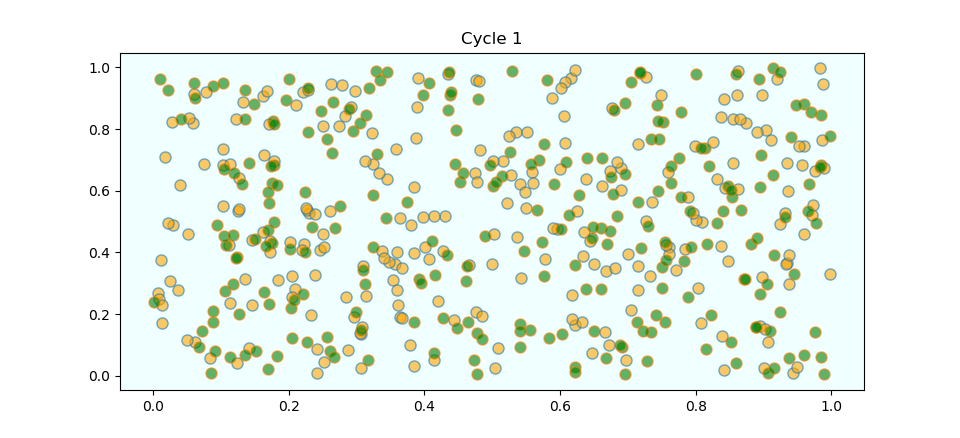
\includegraphics[scale=0.5]{segregation_1}
	\caption{Schelling's Segregation Model: Cycle 1}
	\label{SSM1_ch1}
\end{figure}

\begin{figure}[h!]
	\centering
	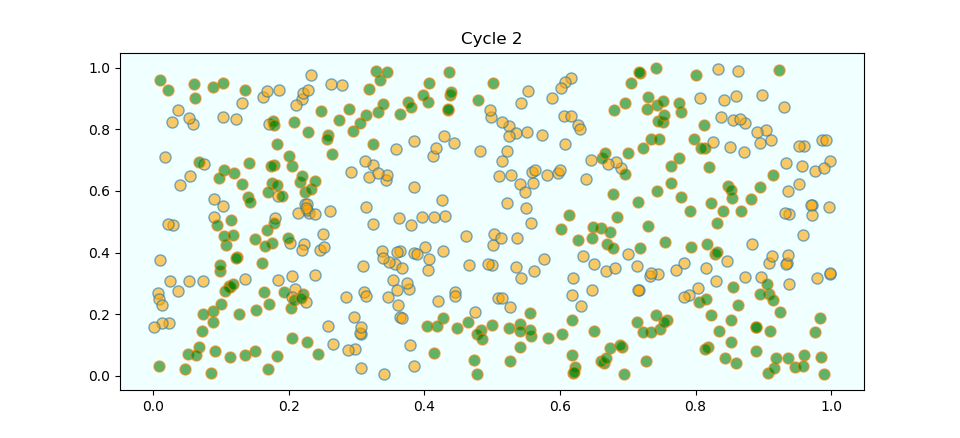
\includegraphics[scale=0.5]{segregation_2}
	\caption{Schelling's Segregation Model: Cycle 2}
	\label{SSM2_ch1}
\end{figure}
\begin{figure}[h!]
	\centering
	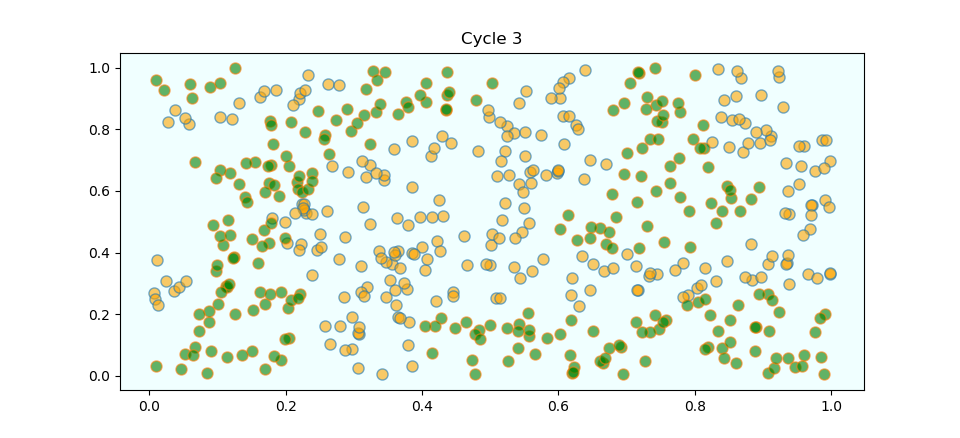
\includegraphics[scale=0.5]{segregation_3}
	\caption{Schelling's Segregation Model: Cycle 3}
	\label{SSM3_ch1}
\end{figure}
\begin{figure}[h!]
	\centering
	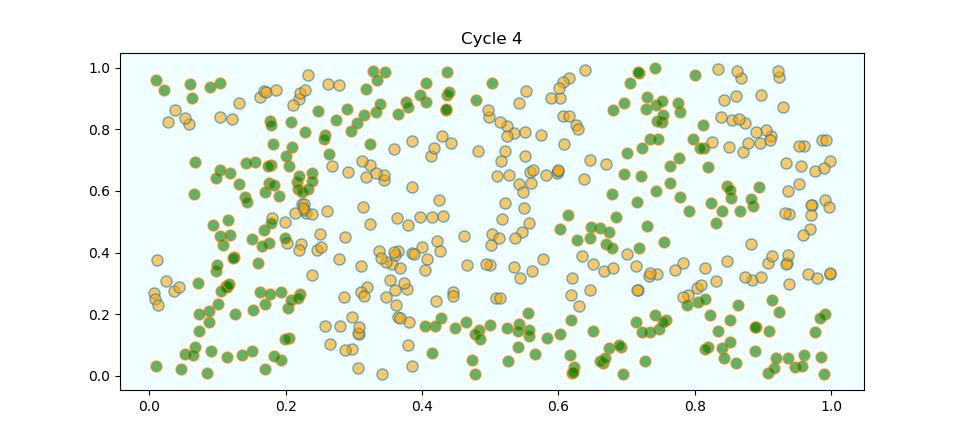
\includegraphics[scale=0.5]{segregation_4}
	\caption{Schelling's Segregation Model: Cycle 4}
	\label{SSM4_ch1}
\end{figure}
\begin{figure}[h!]
	\centering
	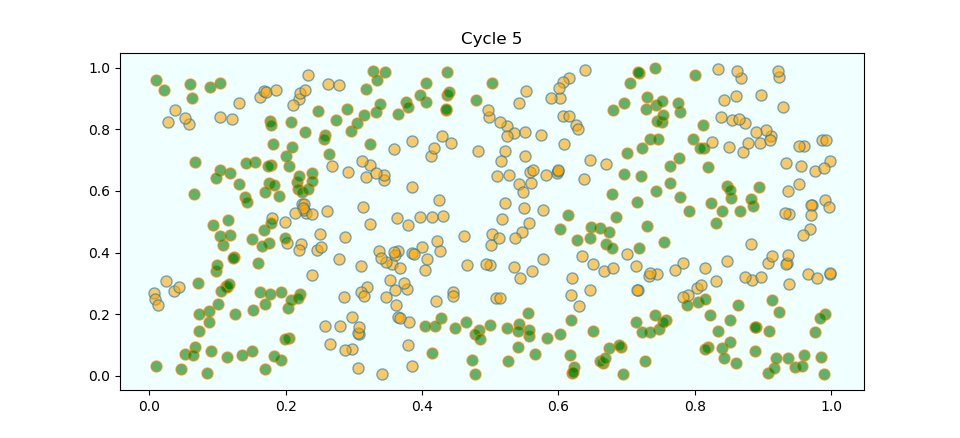
\includegraphics[scale=0.5]{segregation_5}
	\caption{Schelling's Segregation Model: Cycle 5}
	\label{SSM5}
\end{figure}

As can be seen, in cycle 1 (Figure \ref{SSM1_ch1}), the agents are well distributed among each other, but as they move in cycles 2-5, they become progressively more segregated. After 5 cycles all agents are happy and the simulation terminates. With very few assumptions about the agents' preferences, we can see the resulting emergent behavior of segregated neighborhoods in the system as a whole. Not only that, but the agents naturally move to an equilibrium as they adjust their behavior to what their neighbors are doing (\cite{Sargent2019}). 

Agent based modeling has been used to build and understand much more complicated systems then the example illustrated above. The Santa Fe Institute in New Mexico is one of the main proponents of agent based modeling releasing a manifesto supporting using it to understand the "complexity" of economics from the ground up (\citealp{Backhouse2016}). They built the Santa Fe Artificial Stock Market in the 1990's to try and simulate the behavior of agents on the stock market and how they adapt their adapting trading strategies effects the outcome of the market. This is one of the first examples of agents learning and adapting to their environments as part of the model (\cite{LeBaron2002}). In this model agents used a genetic algorithm to adapt their trading strategy at each period by modifying a string (for example $00011100$) where each bit in the string told the agent to use a certain behavior or not. Those trading strategies that did well were coded to survive longer where the agents with worse strategies would randomly modify their own or take a more successful agents strategy (\cite{Arthur1992}). This was supposed to be representative of the learning of traders on the stock market so that the insights taken from running these agents in simulation could be applied to learn something about the real world. 

The authors of Santa Fe Stock Market paper at the time suggested that this was one of many algorithms that could be used to stand in for human behavior saying that reinforcement learning or deep learning could also be used to stand in for human intelligence\footnote{Reinforcement learning is when an algorithm plays a game repeatedly and updates its beliefs about what actions will lead to the best payoff. Deep learning uses deep neural networks to try and estimate the best outcomes in a fashion similar to regression.} (CITATION NEEDED, This was in Shareen Joshi's thesis and in one of their papers, but I am having trouble tracking down the quote. Will use her thesis to find original source or remove reference). Recent research in the field as well as in the field of multi-agent systems, a similar branch of computer science suggest that this is not the case. Because these simulations have agents competing in non-stationary environments that are changing from the perspective of any individual agent every time some other agent changes their behavior, the choice of algorithm dramatically changes how the system behaves (\cite{Rejeb2005}, \cite{Shoham2008}). Further, research that has compared the behavior of human agents in strategic settings to that of these algorithms have found that there is no general algorithm that best approximates human learning(\cite{Tesfatsion2002}). From situation to situation, different algorithms more appropriately behave like humans. This is a problem only assuming that you want your agents to in some way represent human behavior, we might simply want our agents to represent the "rational choice" in any given situation. These algorithms aren't necessarily doing that either. As Holland and Miller say in their 1991 paper "Artificial Adaptive Agents in Economic Theory", "Usually there is only one way to be fully rational, but there are many ways to be less rational." The way they suggest to get around this is to try and build models that have robust behavior across algorithm choice. This is probably not true for their own artificial stock market as it is not even robust across the choice of parameters to program the market. The literature of game theory provides a nice solution to this. The no-regret algorithms they use have the simple property of doing better in the long run than fixing their strategy randomly in the beginning. This is a simple learning requirement that means that this kind of algorithm should be more robust across representing human behavior. It also allows us to combine our simulated models and analytical models in a nice way as we can mathematically describe the processes of such algorithms behavior and we can code agents to use algorithms that have that behavior. This allows the learning process to be less of a black box and instead to be as simple and thus generalizable as possible.

Moving forward this thesis aims to better understand the price of anarchy in auctions by simulating auctions using these no-regret learning algorithms\footnote{these will be discussed in chapter 2, but no-regret learning is a type of reinforcement learning that have certain convergence properties} and seeing how they behave compared to the socially optimal equilibrium. These simulations will try to answer two main questions, what equilibrium do these algorithms converge to (if they converge at all) and what is the calculated price of anarchy in these systems compared to the bounds that theory tells us should exist. Using this framework to explore auctions we will start with a single-item first price auction as it is the best understood theoretically and is the easiest to code. We will then move to simultaneous first price auctions for complementary goods as this is also relatively well understood in terms of the price of anarchy. Finally, time permitting, we will discuss the open question of the price of anarchy in double auctions and discuss how one might go about proving bounds for it.

\chapter{Price of Anarchy in First Price Auctions}
This chapter lays out the mathematical framework for modeling auctions as Bayesian games of incomplete information, formally defines the price of anarchy in auctions, and shows the bounds on the price of anarchy for first price, single payer auctions.

\section{Auctions as Bayesian Game}
Auctions are typically modeled as Bayesian games also known as games with incomplete information. While it is obvious why an auction consisting of the strategic interaction of bidders could be modeled as a game, how it should be modeled requires some thought. After all, while each bidder knows their own valuation of the item being sold, unless for some reason (and against their own interest) the other players announced their valuation of the item before the auction began our bidder will not know how the other players value the item. In fact, it is persicly this lack of information that makes auctions interesting! If all players came into an auction knowing the valuation of other players, for first price, single item auctions the bidder with the highest value would always bid slightly higher than the next highest valuation and win the item (or bid their own valuation if there is a tie for first). Rather it is the uncertainty that players face about the valuation of other players that make things interesting as players must guess how much they should shade their bid (as again no player will ever bid above their valuation) based off of what they know about other players. 

What can we say that bidders know about the valuations of other bidders? Certainly they do not know nothing as we all have reasonable expectations about what some item is worth to others. No one will value a candy bar at a million dollars. But a collector of candy bars might value it at a higher value than an ordinary person who just want to eat the candy bar. For each, could say that this bidder has a probability distribution from which they are drawing their valuation from that is know to the other bidders. For example we might expect normal people valuation of candy bars to be a normal distribution centered at \$1, but the collectors value might be a leplacian distribution (allowing for more black swan events) centered at \$5. This sort of strategic interaction where the players know the distributions that parameters of the game are drawn from are typically called games of incomplete information, or Bayesian games.
 
\subsection{Bayesian Games}
Bayesian games of incomplete information are games in which one or more of the players don't have "full knowledge" of the game that is being played. Introduced by John C. Harsanyi in 1967, rather than players knowing every parameter of the game situation such as utility functions, possible strategies, and information held by other players, each player knows a probability distribution from which these will be drawn. In his paper, Harsanyi says that this type of game can be thought of as a normal game, where "nature" goes first drawing from these probability distributions and assigning values before play begins without the players knowing which specific variation of the game they are playing (TODO CITE Harsanyi). Importantly, each player does know the probability distributions from which each value is selected. Formally such games are defined as follows, 

\begin{dfn}
	A game with incomplete information, also known as a Bayesian game where there are $I$ players, $G = (\Theta, S, P, u)$ consists of:
	\begin{enumerate}
		\item A set $\Theta = \Theta_1 \times \ldots \times \Theta_I$, where $\Theta_i$ is the finite set of possible types for player $i$.
		\item A set $S = S_1 \times \ldots \times S_I$, where $S_i$ is the set of possible strategies for player $i$
		\item A joint probability distribution $p(\theta_1, \dots , \theta_I)$ over types. For finite type space, assume that $p(\theta_i) > 0$ for all $\theta_i \in \Theta_i$
		\item Payoff functions $u_i : S \times \Theta \rightarrow \mathbb{R}$
	\end{enumerate} 
\end{dfn} (TODO CITE Levin)

Using this definition to model our auction the types of players will consist of the publically known distribution from which they are drawing their valuation. That is, our auction will consist of bidders who know their own valuation of the item being bidded on, and the distribution from which each of the other players is drawing their own valuations. In a first price, single item auction if player $i$ wins with bid $b_i$, we define their payoff the winner to be $u_i = v_i - b_i$, the difference between their valuation and their bid and the losers all get $u_i = 0$ since they did not receive the item. Now, a strategy for a player is a function $s_i \in S_i$ that maps a valuation $v_i$ in support of $\Theta_i$ to a bid $s_i(v_i)$. 

Now, we move to the idea of equilibrium in this system. In games of complete information the central equilibrium concept is usually a Nash equilibrium, the set of strategies for all players in which each individual player cannot increase their utility by deviating from their strategy given the strategy of all the other players. This concept is now updated to give us a Bayes-Nash equilibrium where we must also incorporate the distributions for which players are drawing from. 

\begin{dfn}
	A strategy profile constitutes a Bayes-Nash equilibrium if for every player $i$ and every valuation $v_i$ that the player might have, the player chooses a bid $s_i(v_i)$ that maximizes her conditional expected utility where the expectation is over the valuations of the other players, conditioned on a bidder i's valuation being $v_i$. We express that as an equation below.
\end{dfn}

\subsection{Formally Defining First Price Auctions}
NOTE: This section needs cleaning up since it is going to give a lot of duplicate information or redefine things slightly differently from previous sources.

To analyze an first price auction as a game, we give the notation we will be using. This notation comes from Roughgarden et. al 's 2018 (TODO check date) survey of the subject of the price of anarchy in auctions. For a bid profile $\textbf{b} = (b_1, \ldots, b_n)$, we let 
\[
	x_i(\textbf{b}) =
	\begin{cases}
		1 & \text{if player $i$ is the winner} \\
		0 & \text{otherwise}
	\end{cases}
\].

We let $p(\textbf{b}) = \max_{i \in \{1, \ldots, n\} } b_i$ denote the selling price. The utility that a player $i$ receives when their valuation is $v_i$ is 
$$u_i(\textbf{b}; v_i) = (v_i - b_i) \cdot x_i(\textbf{b})$$. 

Now, for a strategy profile $\textbf{s} = (s_1, \ldots, s_n)$, where each $s_i$ is a function for player $i$'s valuation $v_i$ to their bid. We let $\textbf{s}(\textbf{v})$ denote the strategy vector resulting from the vector of valuations $\textbf{v}$. For any given vector $\textbf{x}$, we use $\textbf{x}_{-i}$ to denote the vector $\textbf{x}$ with the $i$th element removed. 

Now, for a first price auction we can say that a strategy profile $\textbf{s} = (s_1, \ldots s_n)$ is a Bayes-Nash equilibrium if and only if 
$$ \mathbb{E}_{\textbf{v}_{-i}} [u_i(\textbf{s} (\textbf{v}); v_i) \ | \ v_i] \geq \EXP_{\valuations_{-i}} [u_i(b^{'}_i, \strategies_{-i}(\valuations_{-i}); v_i) \ | \ v_i] $$.

(TODO cite Roughgarden et al)

\subsection{Example Auction}
We now turn to an example auction to clarify what has just been laid out. In this example we analyze the an auction between two players, Alice and Bob who are bidding on a candy bar where each select their valuations from the uniform distribution $[0,1]$. This is a first price, sealed bid auction where they each submit a bid for the candy bar simultaneously. How are Bob and Alice supposed to decide what to bid on this auction? 

\begin{prop}
	In the first price, sealed bid auction with valuation distributed on $[0,1]$, the unique Bayesian-Nash equilibrium is $\strategies = (s_1(v_1) = v_1 / 2, s_2(v_2) = v_2 / 2)$.
\end{prop}

To show this first, we show that each player is using a best response. First, we note that We calculate that the expected value for player one is,

\begin{align*}
	\EXP_{\valuations_{-1}} [u_1(\strategies(\valuations); v_1 \ | \ v_1)] &= \EXP_{v_2}[u_1( \ s_1(v_1), s_2(v_2); \ v_1 \ | \ v_1)] \\
	&= (v_1 - b_1) \Pr[s_2(v_2) < b_1] + \frac{1}{2}(v_1 - b_1)\Pr[s_2(v_2) = b_1].
\end{align*}

since player expect to get their full utility with the probability that they outbid the other player, and expect to get one half that if they tie with the other bidder (since ties are broken with a coin toss). Now, assuming that player one does not over bid, we know that $b_1 \in [0, \frac{1}{2}]$.

... I'm not sure if I need this

\subsection{Efficiency of First Price Auctions}
Examples of the Bayes-Nash equilibrium have been solved for various combinations of the number of players and distributions from which they draw their valuations. With $n$ bidders it has been shown that the Bayes-Nash equilibrium strategy vector is $s_i(v) = \frac{n-1}{n} v$ for all players. Here the equilibrium is easy to calculate and efficient (meaning that the item will always be allocated to the player with the highest valuation). This is however not always the case. For example if we conduct an auction with two bidders, one choosing from the uniform distribution $[0,1]$ and the other from the uniform distribution $[0,2]$ it has been shown that the Bayes-Nash equilibrium for this auction is:
\begin{align*}
	&s_1(v_1) = \frac{4}{3 v_1} \left(1 - \sqrt{1 - \frac{3v_1^2}{4}}\right)\\
	&s_2(v_2) = \frac{4}{3 v_1} \left(\sqrt{1 + \frac{3v_1^2}{4}} - 1 \right)\\
\end{align*}
 
(CITE Krishna, 2002):

Here bidder one knows that bidder two is more likely to to have a higher valuation than them and thus bid higher and so they shade their bid less than bidder two. This can lead to bidder one drawing a lower valuation than bidder two, but outbidding them regardless getting the item. This is inefficient. More over, it has been shown that solving many of these asymmetric Bayes-Nash equilibrium requires finding a solution to a system of partial differential equations many of which have no closed-form solution (CITE Roughgarden). This means that if we expect bidders to do their homework before an auction and choosing their bidding strategy they might not know what to do. Given this, it is extremely hard to characterize or say things about what these solutions look like. However, just because we are not able to give a closed form to what all of these equillibria look like, that does not mean we aren't able to say anything about them. 

\subsection{Price of Anarchy in First Price Auctions}  
To try and get a sense of how inefficient these auctions can be, computer scientists have been applying a concept known as the price of anarchy to analyze these systems. The price of anarchy is a way to compare the social welfare of a system or a game at its best possible value to that of its worst possible equilibrium under strategic play. In the case of an auction the social welfare is the sum of the utilities of the players plus the revenue of the auctioneer.

\begin{dfn}
	The \textit{social welfare} of a bid profile $\bidders$ when the valuation profile is $\valuations = (v_1, \ldots, v_n)$ is 
	$$ SW(\bidders;\valuations) = \sum_{i=1}^{n} v_i \cdot x_i (\bidders)$$
\end{dfn}

The winning bid does not appear in this equation since the winning bidder is paying exactly as much as the auctioneer is getting and this term cancels out of the social welfare function. This means that welfare is maximized when the bidder with the highest valuation is winner. Thus, if we let $x^*_i(\valuations)$ be an indicator variable for whether or not a player $i$ is the player with the highest valuation (ties broken arbitrarily), the maximum possible social welfare in a single-item auction is 
$$ \OPT(\valuations) = \sum_{i=1}^{n} v_i \cdot x^*_i (\bidders)$$.

Now, that we mathematically describe the social welfare in our system, we can define the price of anarchy. 

\begin{dfn}
	The \textit{price of anarchy} of an auction, with a valuation distribution $\mathcal{F}$ (TODO reconcile notation), is the smallest value of the ratio
	$$ \frac{\EXP_{\valuations} [SW(\strategies(\valuations);\valuations)]}{\EXP_{\valuations}[\OPT(\valuations)]}$$,
	ranging over all Bayes-Nash equilibrium $\strategies$ of the auction.
\end{dfn}

The price of anarchy for the first price auction format is then the worst possible price of anarchy for any choice of the number of players $n$ or valuation distributions $\mathcal{F}$ (TODO: reconcile notation). We can see that the price of anarchy is a number between $0$ and $1$, and that the closer it is to one, the "better" we can guarantee the system's social welfare will be\footnote{Much of the literature for POA (including the paper introducing the idea) defines it as the opposite ratio, Optimal/Worst-EQ where smaller values indicate better systems. For some reason the auction literature defines it in the way I did, so I will remain consistent with them.}.

Incredibly, bounds on the price of anarchy for the format of first-price auctions have been found. Again, this allows us to characterize how much worse the social welfare for the system could be at (Bayes-Nash) equilibrium no matter how many players we have or what distributions they are choosing their valuations from. This sort of guarantee is incredible, especially for systems where we may not want, or it may not be feasible to have a central authority pre-calculate the way to optimize social welfare in a system. Rather, we can trust that the system will perform at least so well under strategic interaction.

\chapter*{Conclusion}
         \addcontentsline{toc}{chapter}{Conclusion}
	\chaptermark{Conclusion}
	\markboth{Conclusion}{Conclusion}
	\setcounter{chapter}{4}
	\setcounter{section}{0}
	
Here's a conclusion, demonstrating the use of all that manual incrementing and table of contents adding that has to happen if you use the starred form of the chapter command. The deal is, the chapter command in \LaTeX\ does a lot of things: it increments the chapter counter, it resets the section counter to zero, it puts the name of the chapter into the table of contents and the running headers, and probably some other stuff. 

So, if you remove all that stuff because you don't like it to say ``Chapter 4: Conclusion'', then you have to manually add all the things \LaTeX\ would normally do for you. Maybe someday we'll write a new chapter macro that doesn't add ``Chapter X'' to the beginning of every chapter title.

\section{More info}
And here's some other random info: the first paragraph after a chapter title or section head \emph{shouldn't be} indented, because indents are to tell the reader that you're starting a new paragraph. Since that's obvious after a chapter or section title, proper typesetting doesn't add an indent there. 


%If you feel it necessary to include an appendix, it goes here.
    \appendix
      \chapter{The First Appendix}
      \chapter{The Second Appendix, for Fun}


%This is where endnotes are supposed to go, if you have them.
%I have no idea how endnotes work with LaTeX.

  \backmatter % backmatter makes the index and bibliography appear properly in the t.o.c...

% if you're using bibtex, the next line forces every entry in the bibtex file to be included
% in your bibliography, regardless of whether or not you've cited it in the thesis.
    \nocite{*}

% Rename my bibliography to be called "Works Cited" and not "References" or ``Bibliography''
% \renewcommand{\bibname}{Works Cited}

%    \bibliographystyle{bsts/mla-good} % there are a variety of styles available; 
%  \bibliographystyle{plainnat}
% replace ``plainnat'' with the style of choice. You can refer to files in the bsts or APA 
% subfolder, e.g. 
 \bibliographystyle{APA/apa-good}  % or
 \bibliography{thesis}
 % Comment the above two lines and uncomment the next line to use biblatex-chicago.
 %\printbibliography[heading=bibintoc]

% Finally, an index would go here... but it is also optional.
\end{document}
